\documentclass[11pt]{beamer}

\usetheme{metropolis}

\usepackage{graphicx}
\usepackage{physics}
\usepackage{adjustbox}
\usepackage{caption}
\usepackage{chemformula}
\usepackage{quoting}
\usepackage[style=chem-angew,backend=bibtex]{biblatex}
\bibliography{references}
%
% Choose how your presentation looks.
%
% For more themes, color themes and font themes, see:
% http://deic.uab.es/~iblanes/beamer_gallery/index_by_theme.html
%
\mode<presentation>
{
  \usetheme{default}      % or try Darmstadt, Madrid, Warsaw, ...
  \usecolortheme{default} % or try albatross, beaver, crane, ...
  \usefonttheme{default}  % or try serif, structurebold, ...
  \setbeamertemplate{navigation symbols}{}
  \setbeamertemplate{caption}[numbered]
  \setbeamerfont{footnote}{size=\tiny}
} 

\usepackage[english]{babel}
\usepackage[utf8]{inputenc}
\graphicspath{{image/}{../lectureMW/image}}

\AtBeginSection[]{
\begin{frame}{Outline}
  \tableofcontents[currentsection]
\end{frame}
}

\title{Lab Review}
\institute{Chemistry Department, Cypress College}
\date{Nov 28, 2022}

\begin{document}

\begin{frame}
  \titlepage
\end{frame}

\begin{frame}{Class Announcements}
  \textbf{Lab}
  \begin{itemize}
  \item Lab Practicuum Week; Mon - Lab Review
  \item Submit \textbf{All} Lab Assignments...
  \end{itemize}

  \textbf{Lecture}
  \begin{itemize}
  \item Finish up Ch 9; Begin Ch 10 and 11
  \item Final Exam Dec 10th in Lecture
  \item Quiz and Homework posted this Fri, Dec 2nd
  \end{itemize}
\end{frame}

\section{Lab Review}

\begin{frame}{Laboratory Equipment/Check-in}
  \centering
  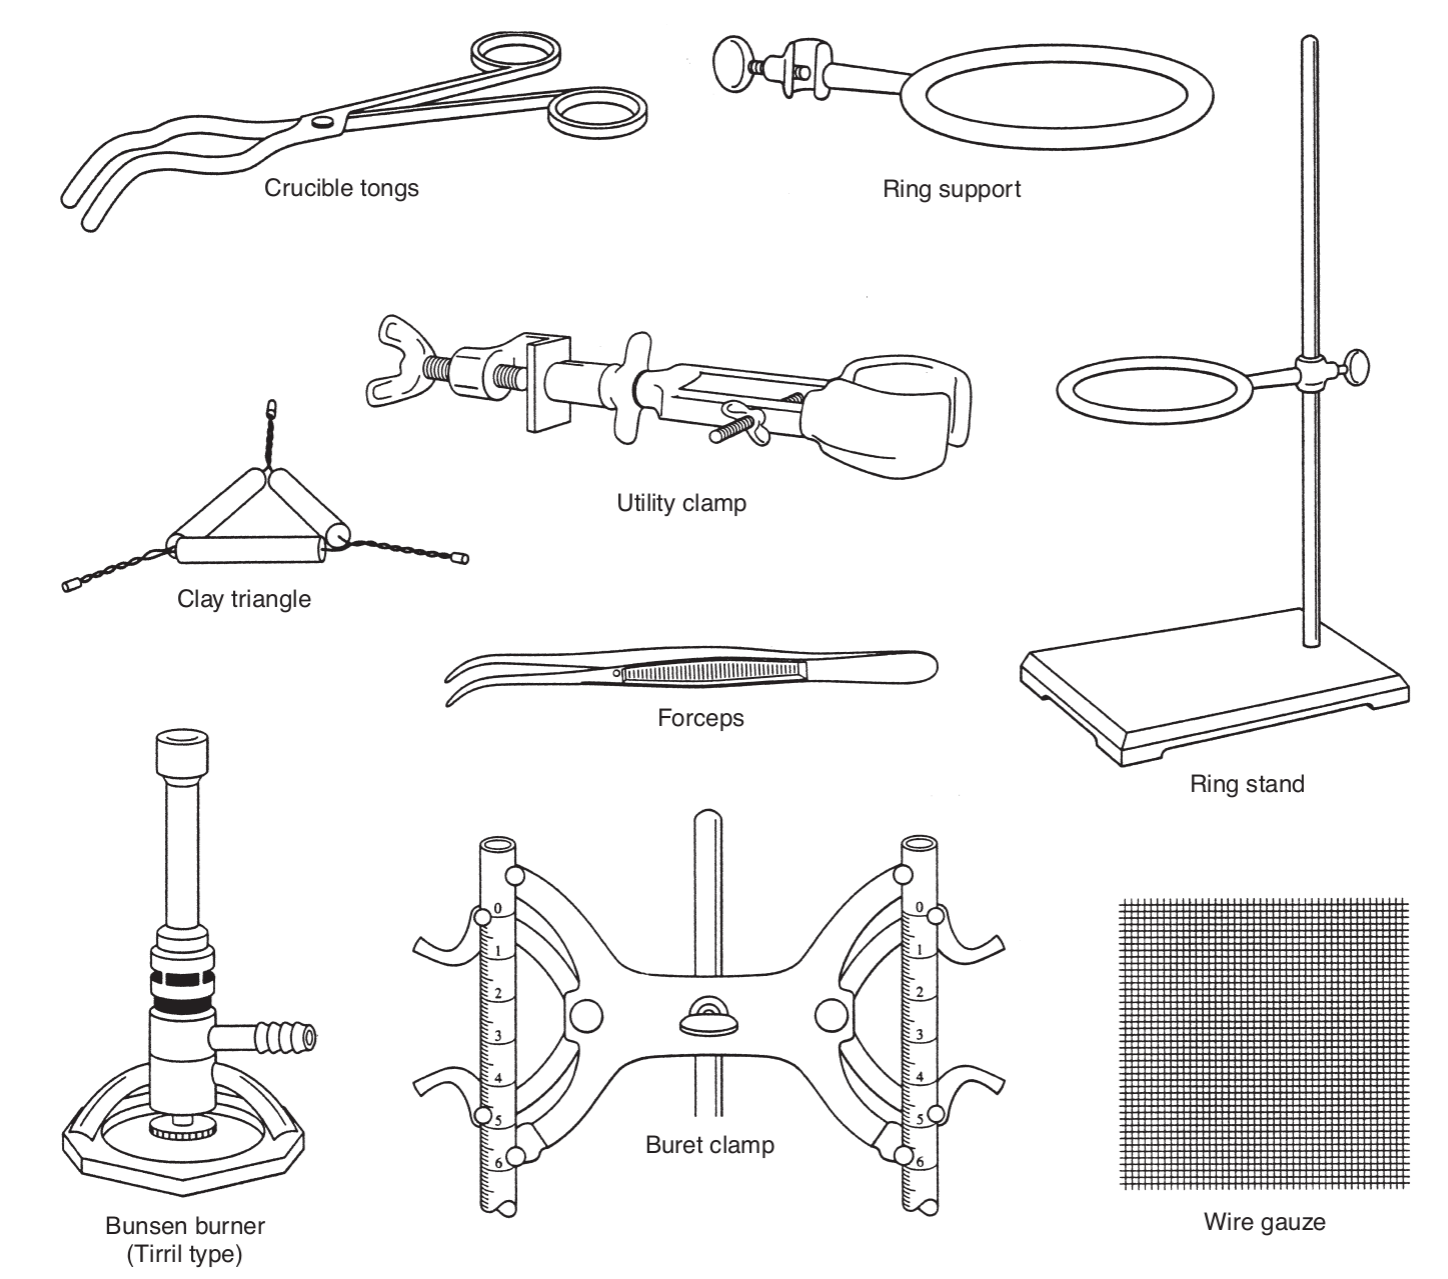
\includegraphics[width=0.8\linewidth]{equip_lab}
\end{frame}

\begin{frame}{Laboratory Equipment/Check-in}
  \centering
  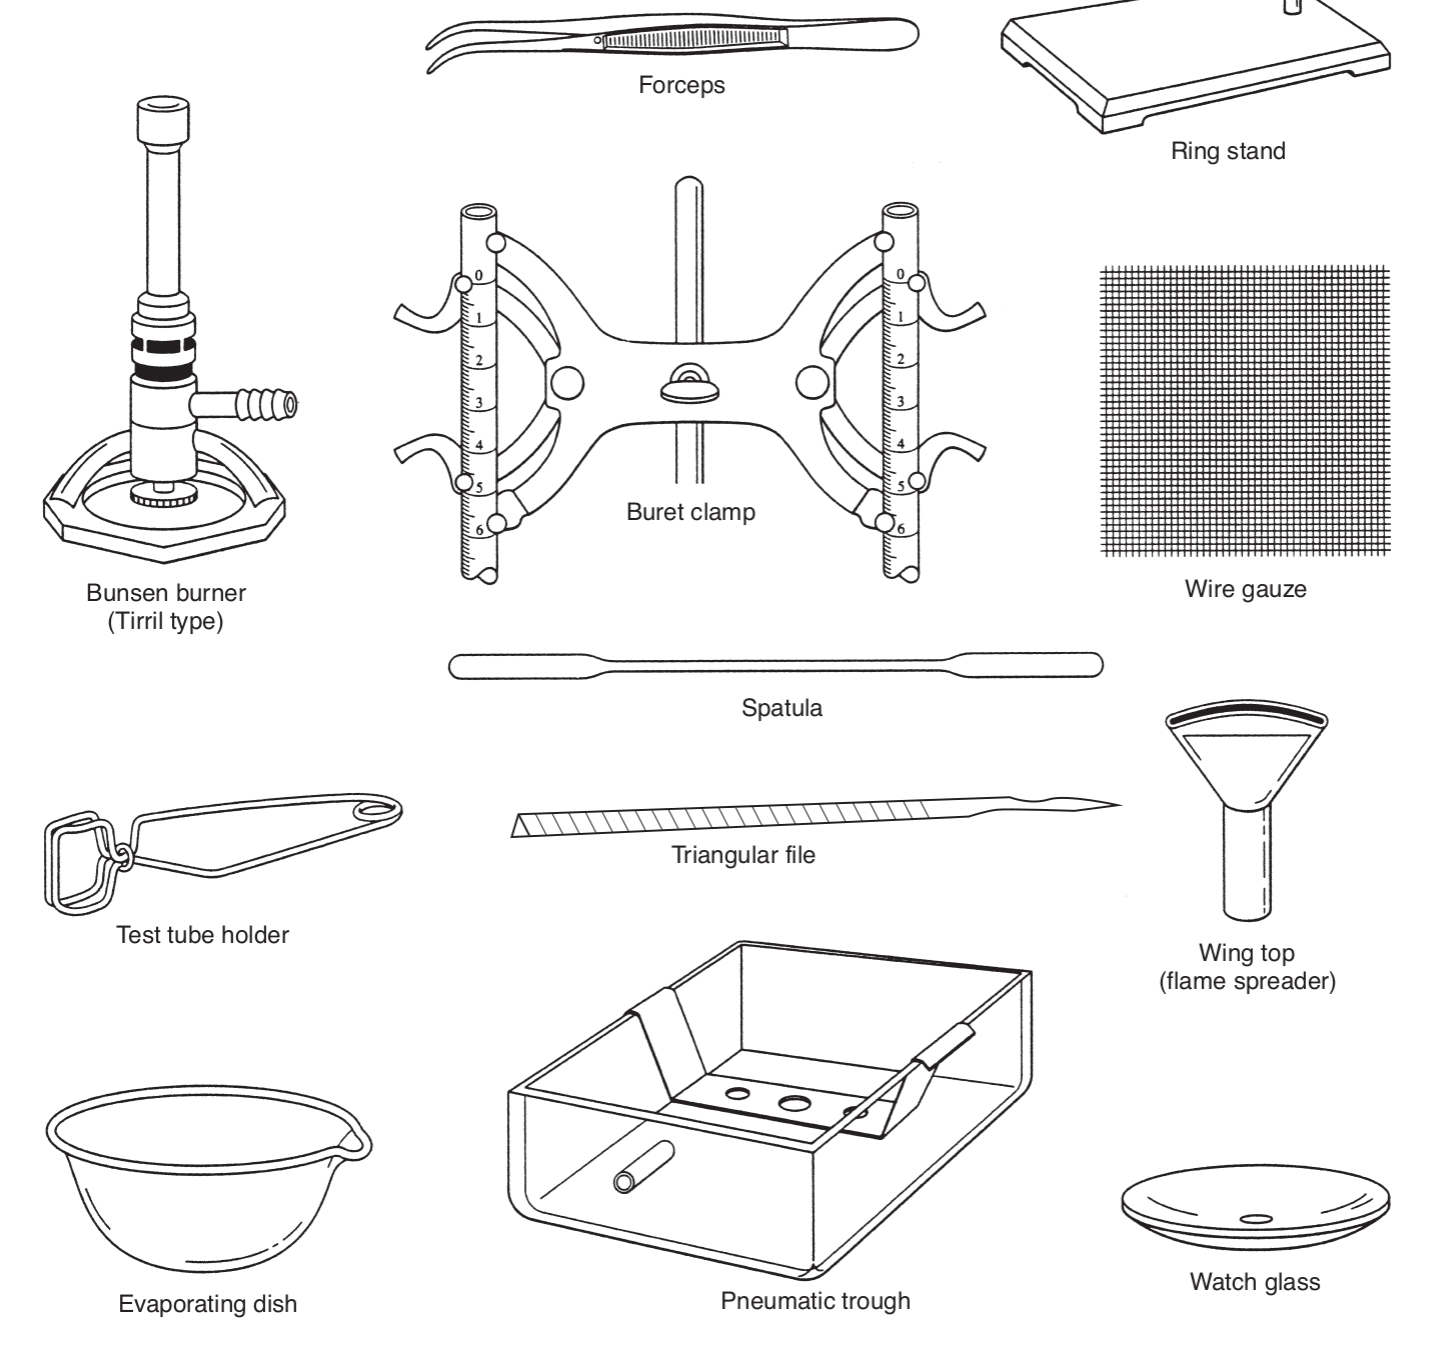
\includegraphics[width=0.8\linewidth]{equip_lab2}
\end{frame}

\begin{frame}{Laboratory Equipment/Check-in}
  \centering
  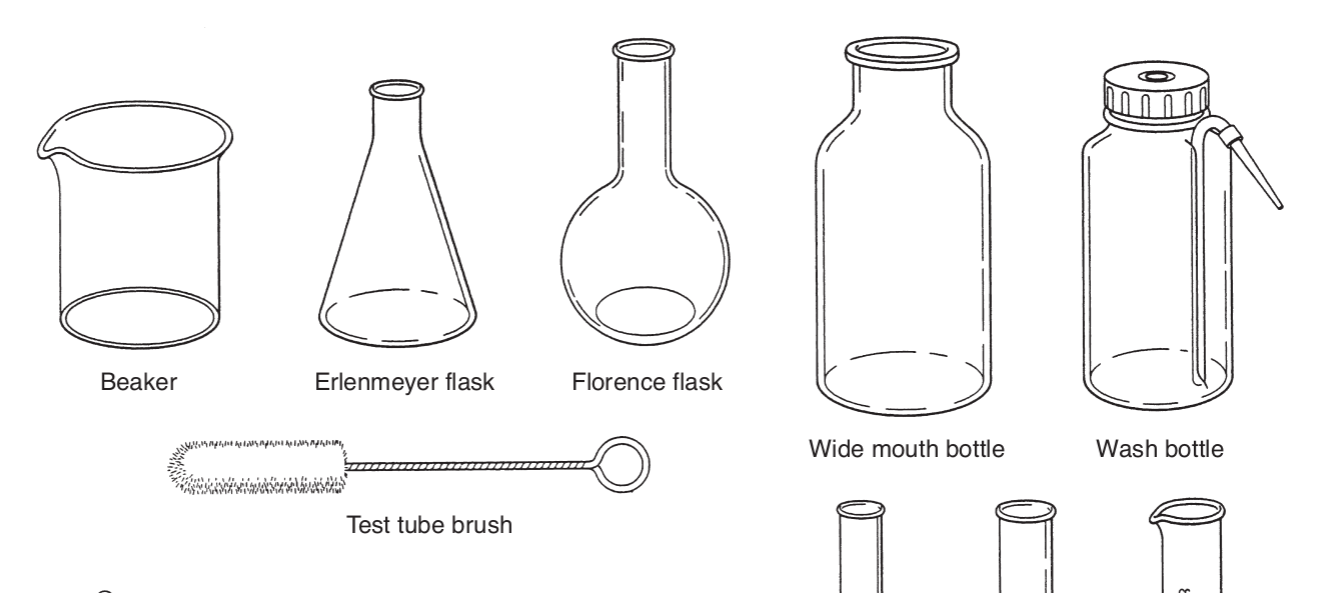
\includegraphics[width=\linewidth]{equip_lab3}
\end{frame}

\begin{frame}{Laboratory Equipment/Check-in}
  \centering
  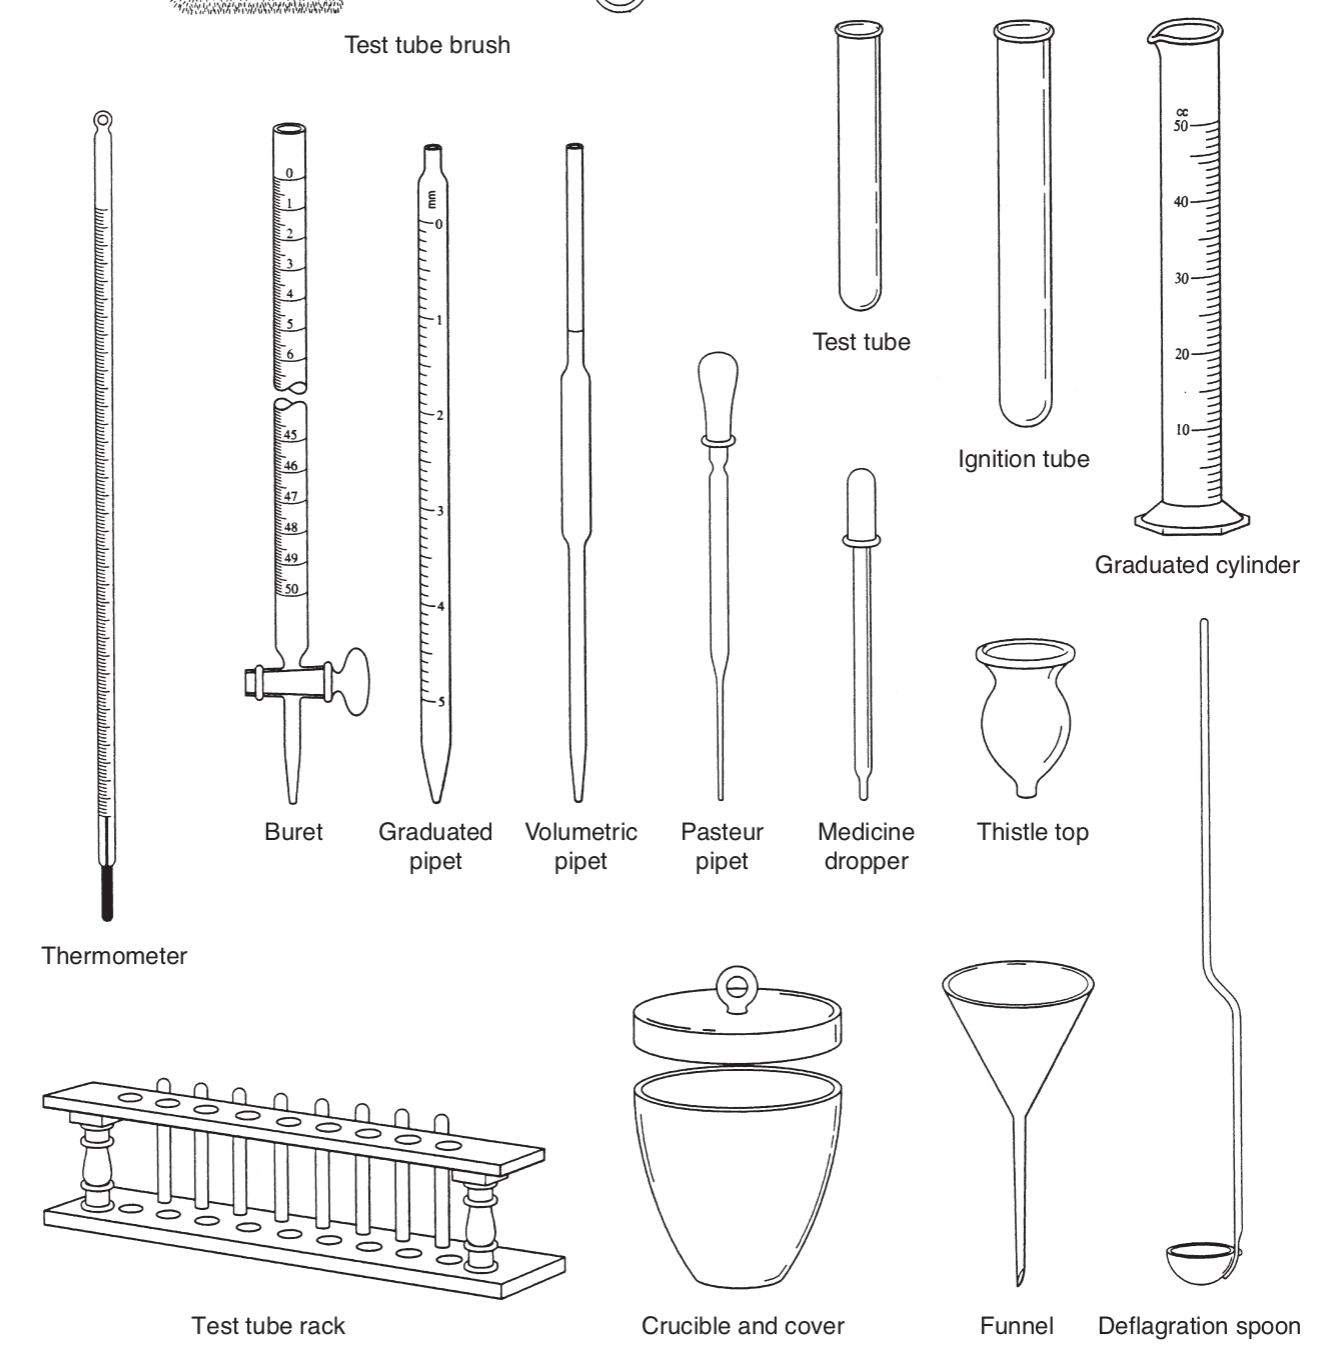
\includegraphics[width=0.7\linewidth]{equip_lab4}
\end{frame}

\begin{frame}{Lab Safety}
  \begin{itemize}
  \item Common sense - lab safety clothing (goggles, long pants),
    no eating/drinking in lab
  \item Familiarize material safety data sheets (MSDS)
  \item Label the reagent bottles and never return reagent back
    into the bottle
  \item Know the locations of the fire extinguisher
  \item Dispose chemicals into waste containers
  \end{itemize}
\end{frame}

\begin{frame}{Math Toolbox}
  \begin{itemize}
  \item Scientific Notation
  \item Significant figures
  \item Unit Conversion
  \end{itemize}
\end{frame}

\begin{frame}{Scientific Notation}
  The scientific notation is expressed
  \begin{equation}
    N = C \times 10^m
  \end{equation}
  where $N$ is a large number, $C$ is the coefficient (a number between $1-9$)
  and $m$ is the exponent (a positive or negative integer)

  \textbf{Example:} $0.00363246 = 3.63246 \times 10^{-3}$

\end{frame}

\begin{frame}{Significant Figures}
  \begin{itemize}
  \item The meaningful digits in a measured or calculated
    quantity
  \item Example: $0.00363246 \simeq 3.63 \times 10^{-3}$ to three
    sig figures
  \item Implies relative accuracy of $10^{-m}$, e.g. $0.1\%$ for $m=3$
  \item[] \begin{center}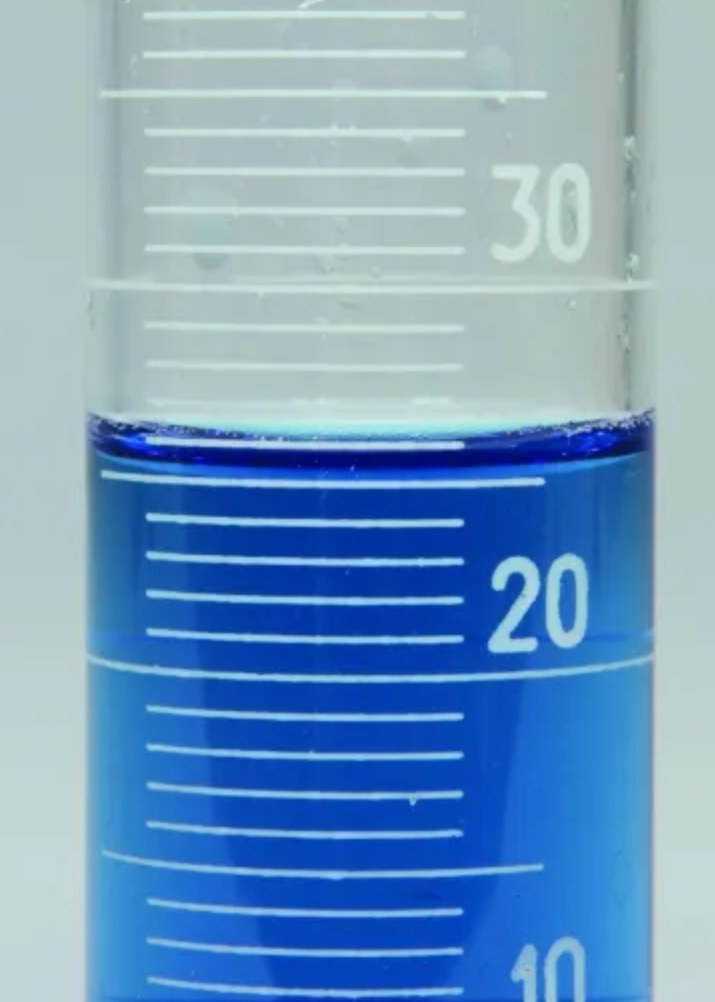
\includegraphics[scale=0.1]{grad}
  \end{center}
  \end{itemize}
\end{frame}

\begin{frame}{Leading, Sandwiched and Trailing Zeroes}
  \textbf{Leading zeroes:} Precede non-zero digits in a
  decimal number are \textbf{not} significant e.g. 0.00001

  \textbf{Sandwiched zeroes:} Occur between nonzero numbers are significant
  e.g. 10,024
  
  \textbf{Trailing zeroes:} Following non-zero numbers are
  significant in numbers with a decimal point e.g. 1,000.
\end{frame}

\begin{frame}{Calculation: Rules for Rounding}
  \textbf{Rule 1:} In carrying out a multiplication or division,
  the answer cannot have more significant figures than either of
  the original numbers.

  \textbf{Example:}
  \begin{equation}
    \frac{278 \text{mi}}{11.70 \text{gal}} = 23.8 \text{mi/gal}
  \end{equation}
  
\end{frame}

\begin{frame}{Calculation: Rules for Rounding}
  \textbf{Rule 2:} In carrying out an addition or subtraction, the
  answer cannot have more digits after the decimal point than either
  of the original numbers or more digits after the leftmost uncertain
  digit than either of the original numbers.

  \textbf{Example:}
  \begin{equation}
    3.18 \text{L} + 0.01315 \text{L} = 3.19 \text{L}
  \end{equation}
\end{frame}

\begin{frame}{Unit Conversion}
  \centering
  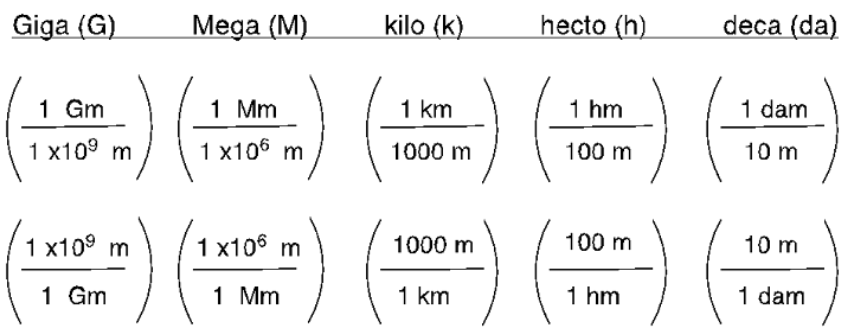
\includegraphics[scale=0.3]{metric_1}
  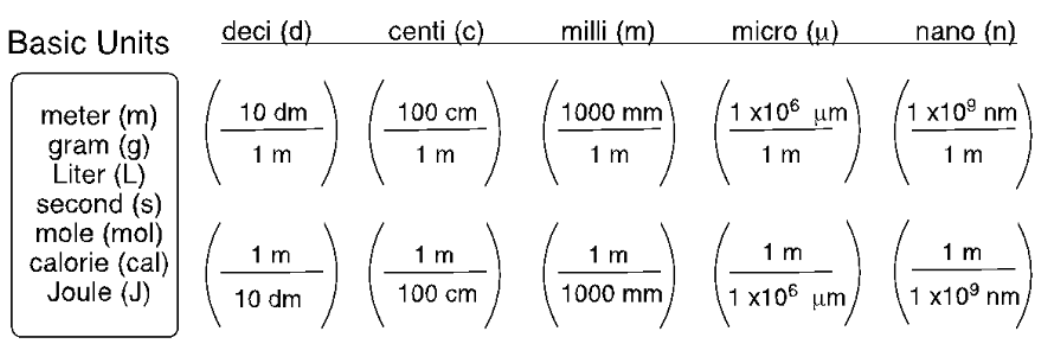
\includegraphics[scale=0.3]{metric_2}
\end{frame}

\begin{frame}{Nomenclature}
  \begin{itemize}
  \item Common mistakes: mixing between ionic and molecular
    compounds e.g. Ca$_3$(PO$_4$)$_2$
  \item Naming ionic compounds, memorize the polyatomic ions
  \item Naming molecular compounds, memorize the prefixes
  \end{itemize}
\end{frame}

\begin{frame}{Naming Binary Ionic Compounds}
  The metal cation is named first, followed by the nonmetal anion.
  The word ion is dropped from both parts.

  \centering
  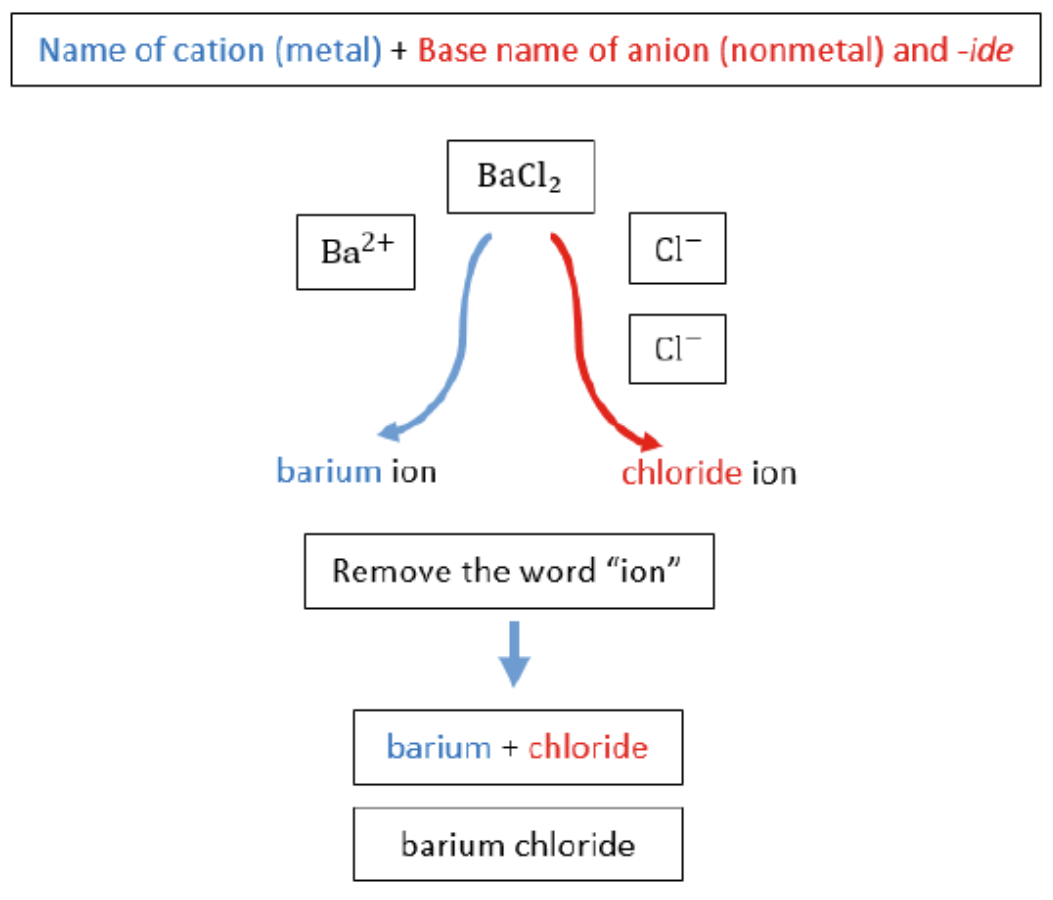
\includegraphics[width=0.7\linewidth]{barium_examp.png}
\end{frame}

\begin{frame}{Naming Molecular Compounds}
  \begin{center}
    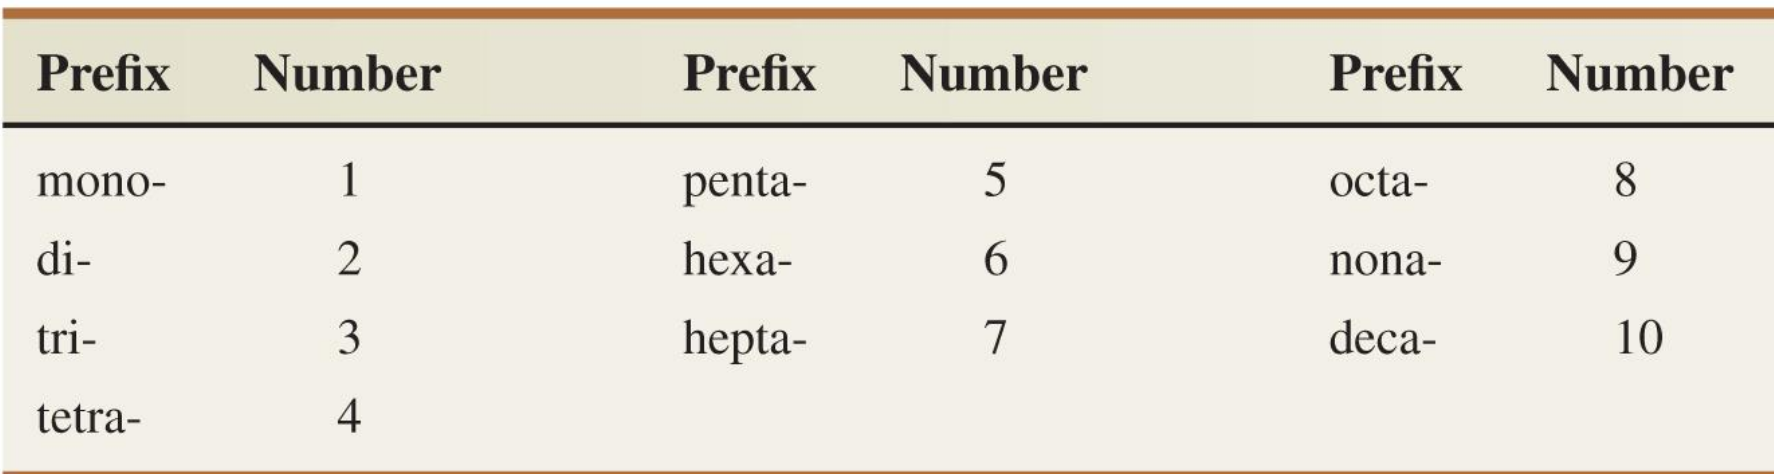
\includegraphics[width=\linewidth]{prefix_name}
  \end{center}
  
  \begin{enumerate}
  \item Use numerical prefix for the element (usually ignore the first
    when using ``mono'')
  \item Add ``-ide'' to the second element
  \end{enumerate}
\end{frame}

\begin{frame}{Laboratory Techniques}
  \begin{itemize}
  \item Bunsen burner
  \item Evaporation
  \item Gravity Filtration
  \end{itemize}
\end{frame}

\begin{frame}{Bunsen Burner}
  \begin{center}
    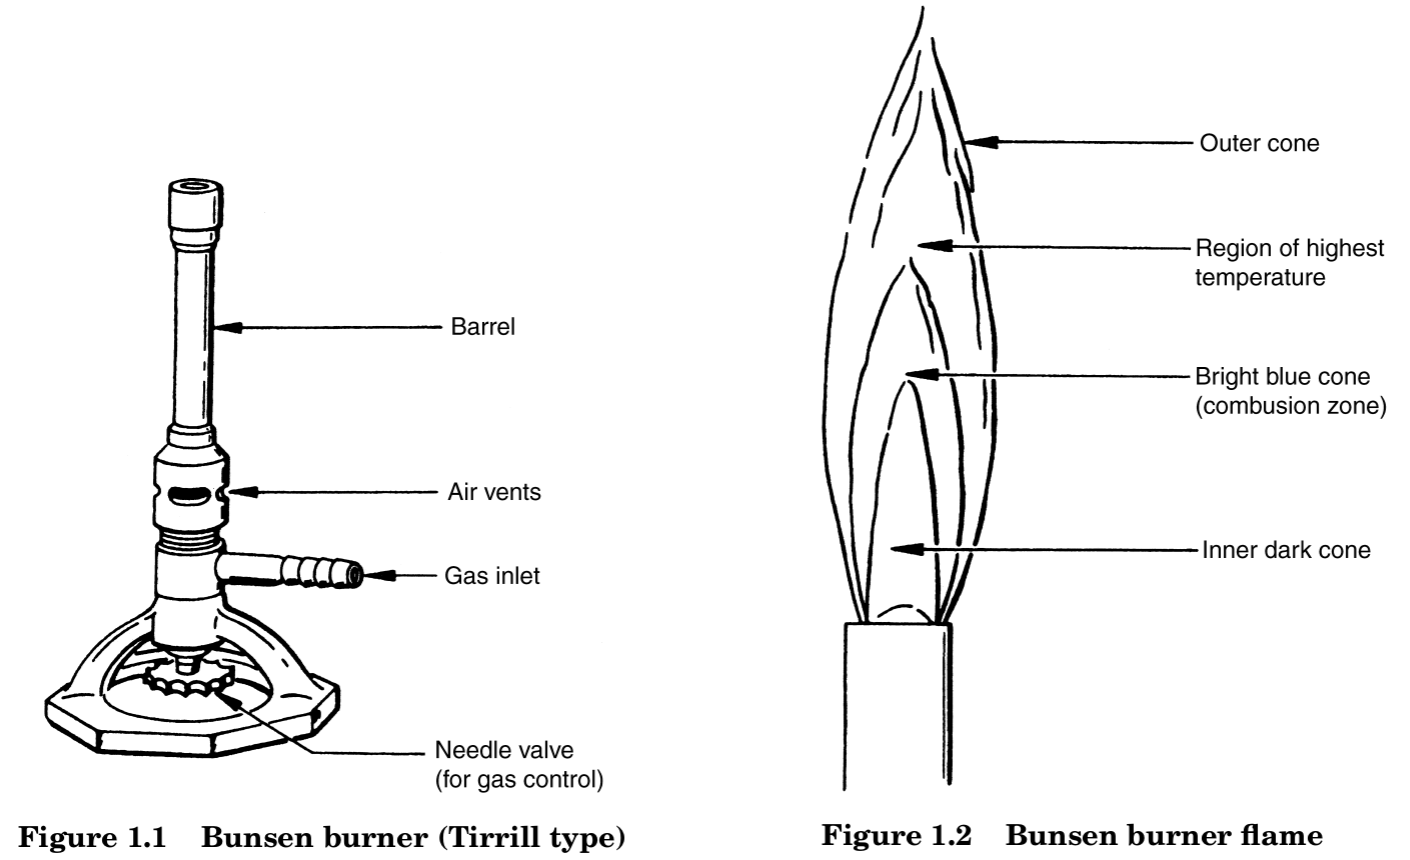
\includegraphics[width=\linewidth]{bunsen_burn}
  \end{center}
\end{frame}

\begin{frame}{Evaporation}
  \begin{center}
    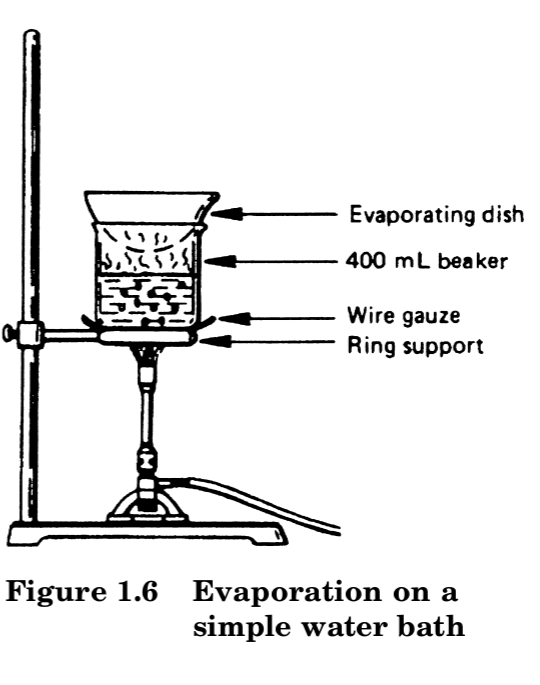
\includegraphics[width=0.5\linewidth]{evap_tech}
  \end{center}
\end{frame}

\begin{frame}{Gravity Filtration}
  \begin{center}
    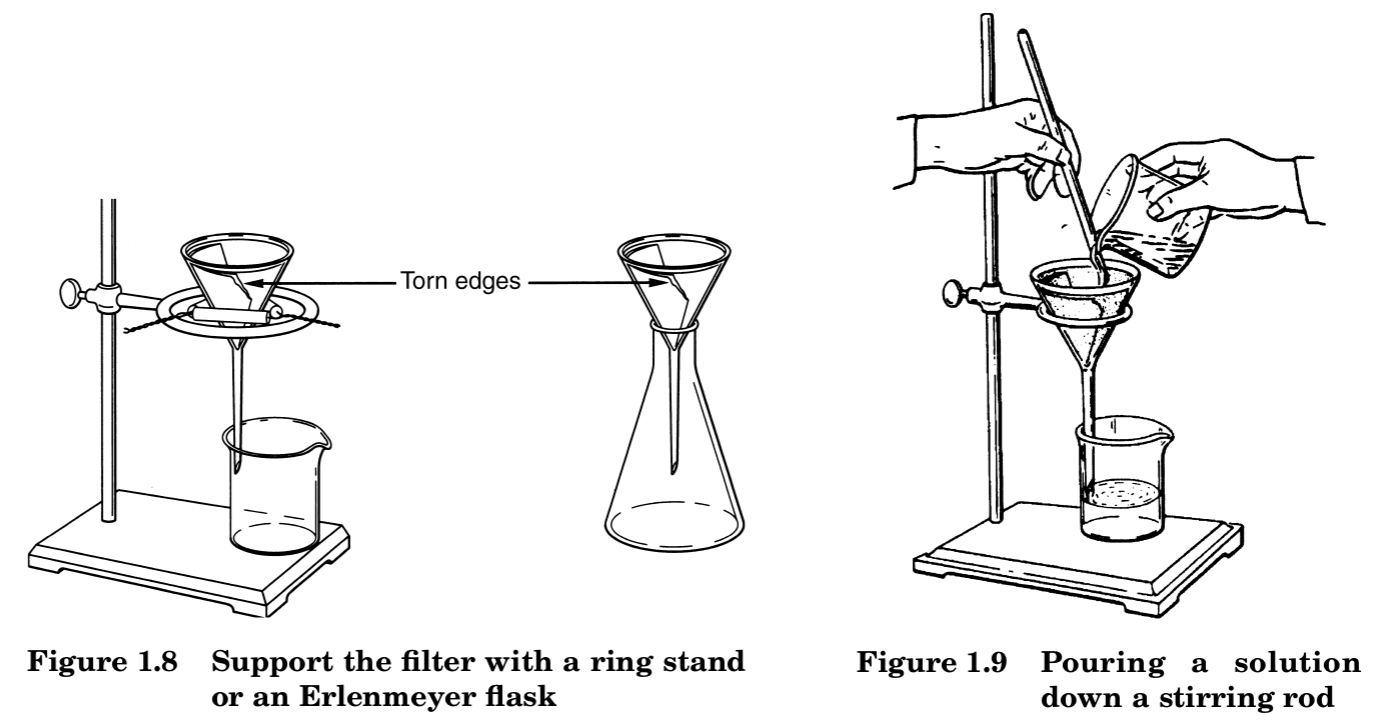
\includegraphics[width=\linewidth]{grav_filt}
  \end{center}
\end{frame}

\begin{frame}{Measurements}
  \begin{center}
    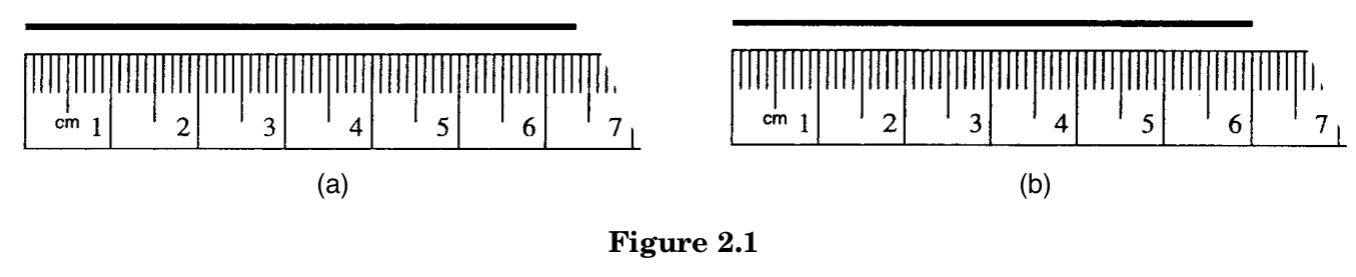
\includegraphics[width=\linewidth]{ruler}\\
    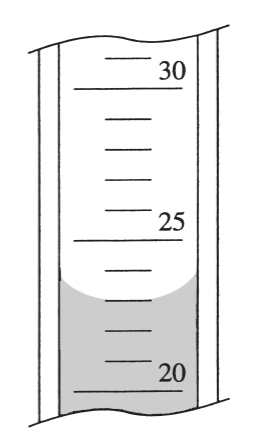
\includegraphics[width=0.2\linewidth]{grad_cycl}
  \end{center}
  Calculations for density (mass/volume)
\end{frame}

\begin{frame}{Water in Hydrates}
  \begin{center}
    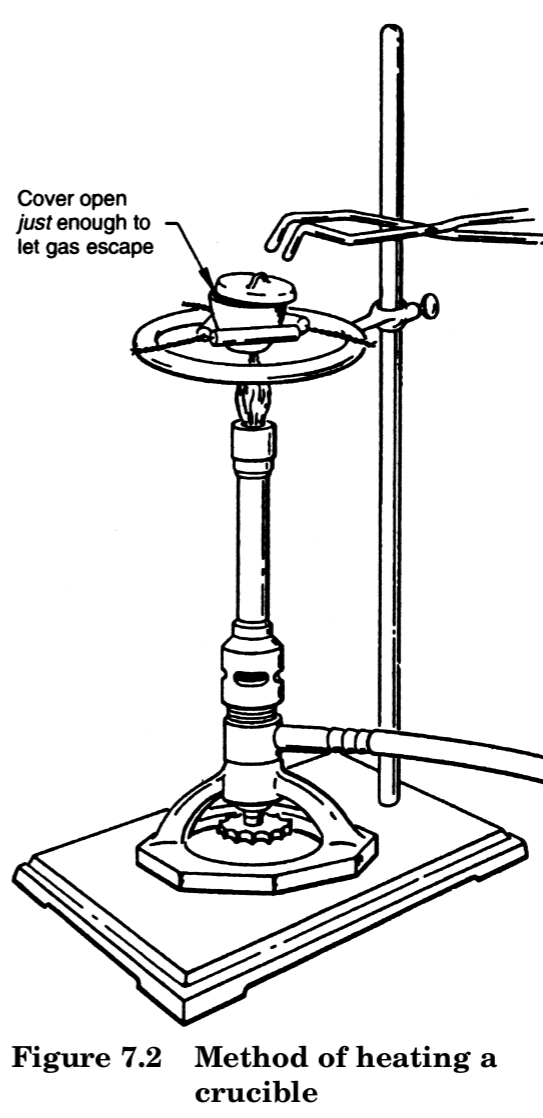
\includegraphics[width=0.35\linewidth]{hydrate}
  \end{center}
\end{frame}

\begin{frame}{Single+Double Displacement Reactions}
  \textbf{Signs for Chemical Reaction}
  
  \begin{itemize}
  \item Color change
  \item Gas formation
  \item Exothermic and endothermic (heat changes)
  \item Precipitation (solid formation) - Solubility rules
  \end{itemize}
\end{frame}

\begin{frame}{Electrolytes}
  \begin{itemize}
  \item Take home message: The formation of ions
  \item Strong electrolytes are solids that dissolve into
    ions
  \item Weak electrolytes are solids that doesn't dissolve into
    ions
  \end{itemize}
\end{frame}

\begin{frame}{KCl Reaction}
  KHCO$_3$(aq) + HCl(aq) $\rightarrow$ KCl(aq) + H$_2$O(l) + CO$_2$(g)

  \begin{itemize}
  \item Understanding the chemical equation e.g. cookbook recipe
  \item Limiting reagent type problem
  \item Determining amount moles HCl from molarity needed to react
    with all your KHCO$_3$(s)
  \end{itemize}
\end{frame}

\begin{frame}{Lewis Structures}
  \begin{enumerate}
  \item Count the total number of valence electrons
  \item Draw the atomic skeleton by determining the central atoms
    (generally the one capable of making many bonds)
  \item Add single bonds (each counts as 2 electrons) to atoms
    and add lone pairs if needed to satisfy the octet rule
  \item Check that if the amount of valence electrons counted match
    the Lewis structure
  \item Check formal charges on the atoms
  \end{enumerate}  
\end{frame}

\begin{frame}{Computing Formal Charges}
  \begin{center}
    Formal Charge = VE - $\frac{1}{2}$ BE - NBE
  \end{center}
  where VE is the number of valence electrons, BE is the bonding
  electron, and NBE is the nonbonding electron aka lone pairs
\end{frame}

\begin{frame}{Resonance Structures}
  As seen in the previous slide, O$_3$ and CO$_3^{-2}$ have multiple
  structures that are valid

  \textbf{Resonance structures} - the movement of electrons satisfying
  a valid Lewis Structure
  
  \centering
  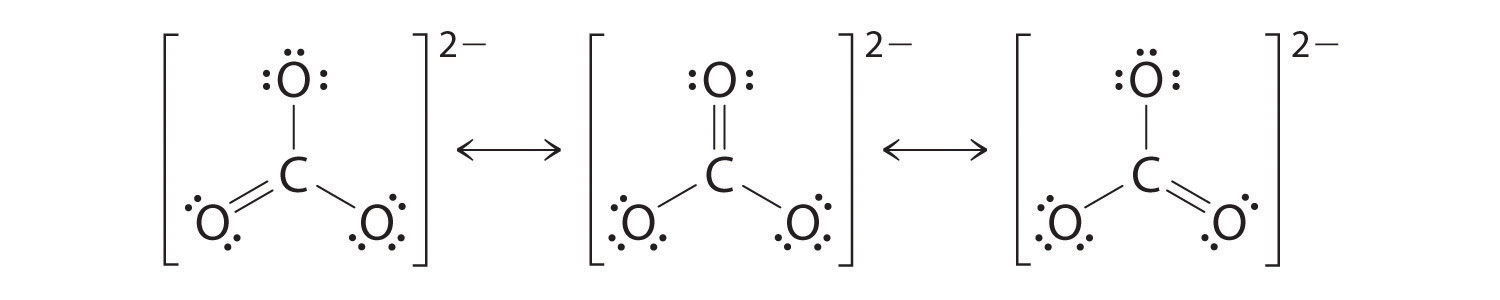
\includegraphics[width=1\linewidth]{resonance_struct}
\end{frame}

\end{document}
